\section{Il protocollo MySQL}
In questo paragrafo verr� analizzato, a grandi linee, il protocollo MySQL\footnote{Maggiori informazioni possono essere prelevate dal sito:\\http://forge.mysql.com/wiki/MySQL\_Internals\_ClientServer\_Protocol}. Questo permetter� di capire in che modo funziona il plugin per l'analisi dei pacchetti MySQL e da dove preleva le informazioni che esporta (l'username dell'utente che si collega al server, il database che sta interrogando, etc\ldots).

� importante notare fin da subito che esistono delle differenze sostanziali tra le versioni minori e quelle maggiori o uguali alla 4.1 del protocollo. Alcune di queste differenze sono trasparenti allo scopo del plugin, altre, come si vedr�, saranno gestite.

\subsection{L'handshake}
Dopo l'handshake a livello TCP, viene effettuato un secondo handshake a livello di protocollo MySQL. In questa fase vengono inviati esattamente i 3 pacchetti\footnote{In questo contesto i pacchetti sono intesi come pacchetti del protocollo MySQL.} seguenti:

\begin{enumerate}
\item Il server, tra le altre cose, informa il client sulla propria versione, sulla versione del protocollo che � in grado di gestire, sul linguaggio accettato e sull'identificativo del thread che gestisce la connessione. Questo pacchetto � conosciuto come \emph{greeting packet}.
\item Il client a sua volta invia al server delle informazioni utili per la connessione, come ad esempio la dimensione massima dei pacchetti, in byte, che � in grado di accettare. Oltre a queste informazioni, invia anche le credenziali dell'utente (username e password) necessarie per l'autenticazione\footnote{L'autenticazione in realt� inizia dal \emph{greeting packet} ed � differente a seconda che vengano usati protocolli inferiori al 4.1 oppure no.}. Per quest'ultimo motivo il pacchetto viene conosciuto come \emph{client authentication packet} o \emph{login packet}. Se entrambi, client e server, gestiscono la versione 4.1 del protocollo\footnote{Si noti che in questa fase, il client sa gi� quale versione del protocollo sar� usata, perch� conosce sia la sua, che quella del server (che gli � stata inviata nel \emph{greeting packet}).}, allora in questo pacchetto il client pu� inviare anche il nome del database sul quale intende lavorare. Ancora, il formato del pacchetto � differente a seconda che si usino delle versioni superiori o uguali alla 4.1 del protocollo, oppure no.
\item Il server conclude l'handshake inviando al client un pacchetto chiamato \emph{result packet}. Se � in grado di soddisfare le richieste del client e l'autenticazione � avvenuta con successo, la connessione va avanti, altrimenti il server nega l'accesso e chiude la connessione.
\end{enumerate}
Sia il server (nel \emph{greeting packet}) che il client (nel \emph{login packet}) inviano una maschera di bit di 2 byte che contiene svariate informazioni, tra cui un flag che indica se sono in grado di gestire il protocollo 4.1 o superiore. La maschera inviata dal server viene chiamata \emph{server\_capabilities}, mentre quella inviata dal client prende il nome di \emph{client\_flag} e, nel caso in cui il protocollo usato � il 4.1 o superiore, dopo \emph{client\_flag} il client invia altri 2 byte conosciuti come \emph{client\_extended\_flag}.

\subsection{L'header dei pacchetti}
Tutti i pacchetti MySQL hanno un'intestazione fissa di 4 byte. I primi 3 byte indicano la dimensione, in byte, del pacchetto stesso e, dato che questa informazione � un numero intero non negativo, la dimensione massima di un pacchetto MySQL � di $2^{24}=16$MB. Ai fini del plugin, questo vuol dire che un pacchetto MySQL pu� essere frammentato in pi� pacchetti TCP.

L'ultimo byte dell'intestazione indica il numero di sequenza del pacchetto. Questo numero viene azzerato alla fine di ogni comunicazione. Quindi, ad esempio, i tre pacchetti dell'handshake sono numerati 0, 1 e 2 e, dopo di ci�, la sequenza viene riazzerata.

\subsection{I pacchetti di richiesta (\emph{command packet})}
Se l'handshake � avvenuto con successo, il client pu� iniziare a interrogare il server inviando dei pacchetti conosciuti come \emph{command packet}. Il primo byte di questo pacchetto identifica il comando, mentre i rimanenti byte ne sono l'argomento.

\subsection{I pacchetti di risposta (\emph{result packet})}
\label{result_packet}
Ricevuta la richiesta dal client, il server risponde con quello che viene chiamato genericamente un \emph{result packet} (come quello che termina l'handshake). Il primo byte di questo pacchetto � chiamato \emph{field\_count} e identifica il tipo di risposta che il server da al client. A seconda del valore del \emph{field\_count} questo pacchetto viene chiamato:

\begin{description}
\item[\footnotesize{Ok Packet:}]{indica che tutto � andato bene, lo si riconosce perch� il \emph{field\_count} � 0x00.}
\item[\footnotesize{Error Packet:}]{indica che c'� stato un errore, lo si riconosce perch� il \emph{field\_count} � 0xFF.}
\item[\footnotesize{Result Set Header Packet:}]{� l'intestazione del risultato di una query. Il \emph{field\_count} ha un valore compreso tra 0x01 a 0xFD e indica il numero di colonne della tabella risultante\footnote{Potrebbe sembrare che il numero di colonne del risultato sia al pi� 253 (0xFD). In realt� questo singolo byte pu� anche indicare quanti byte successivi devono essere presi per calcolare un numero intero che arriva sino a $2^{64}$.}.}
\end{description}
Nel caso di un \texttt{Result Set Header Packet}, il server invier� tutti i pacchetti (incrementando sempre il numero di sequenza) che permetteranno al client di ottenere l'intera tabella del risultato della query. Il server invier� dapprima tanti pacchetti per quanto era il valore del \emph{field\_count} del \texttt{Result Set Header Packet}. Questa prima serie di pacchetti, ognuno dei quali � chiamato \emph{Field Packet}, definisce i campi delle colonne della tabella (ad esempio, id di tipo intero, nome di tipo stringa, etc\ldots). La fine di questa prima serie di pacchetti viene decretata dall'invio del pacchetto chiamato \emph{EOF Packet} (il cui primo byte vale 0xFE) che, a volte, pu� servire per trasportare delle informazioni. Il server quindi invia al client un'altra serie di pacchetti chiamati \emph{Data Packet}, ognuno dei quali contiene una riga della tabella (quindi il valore della prima colonna, il valore della seconda colonna, etc\ldots). Ed infine, per terminare la sequenza dei \emph{Data Packet} il server invia un altro pacchetto di \emph{EOF Packet}.

La figura \ref{mysql-protocol} mostra un esempio di connessione MySQL in cui, dopo l'handshake, il client seleziona un database ed esegue una SELECT. Si noti come, grazie alle informazioni ricevute, il client � in grado di creare la tabella risultante.

\begin{figure}[htbp]
    \centering
    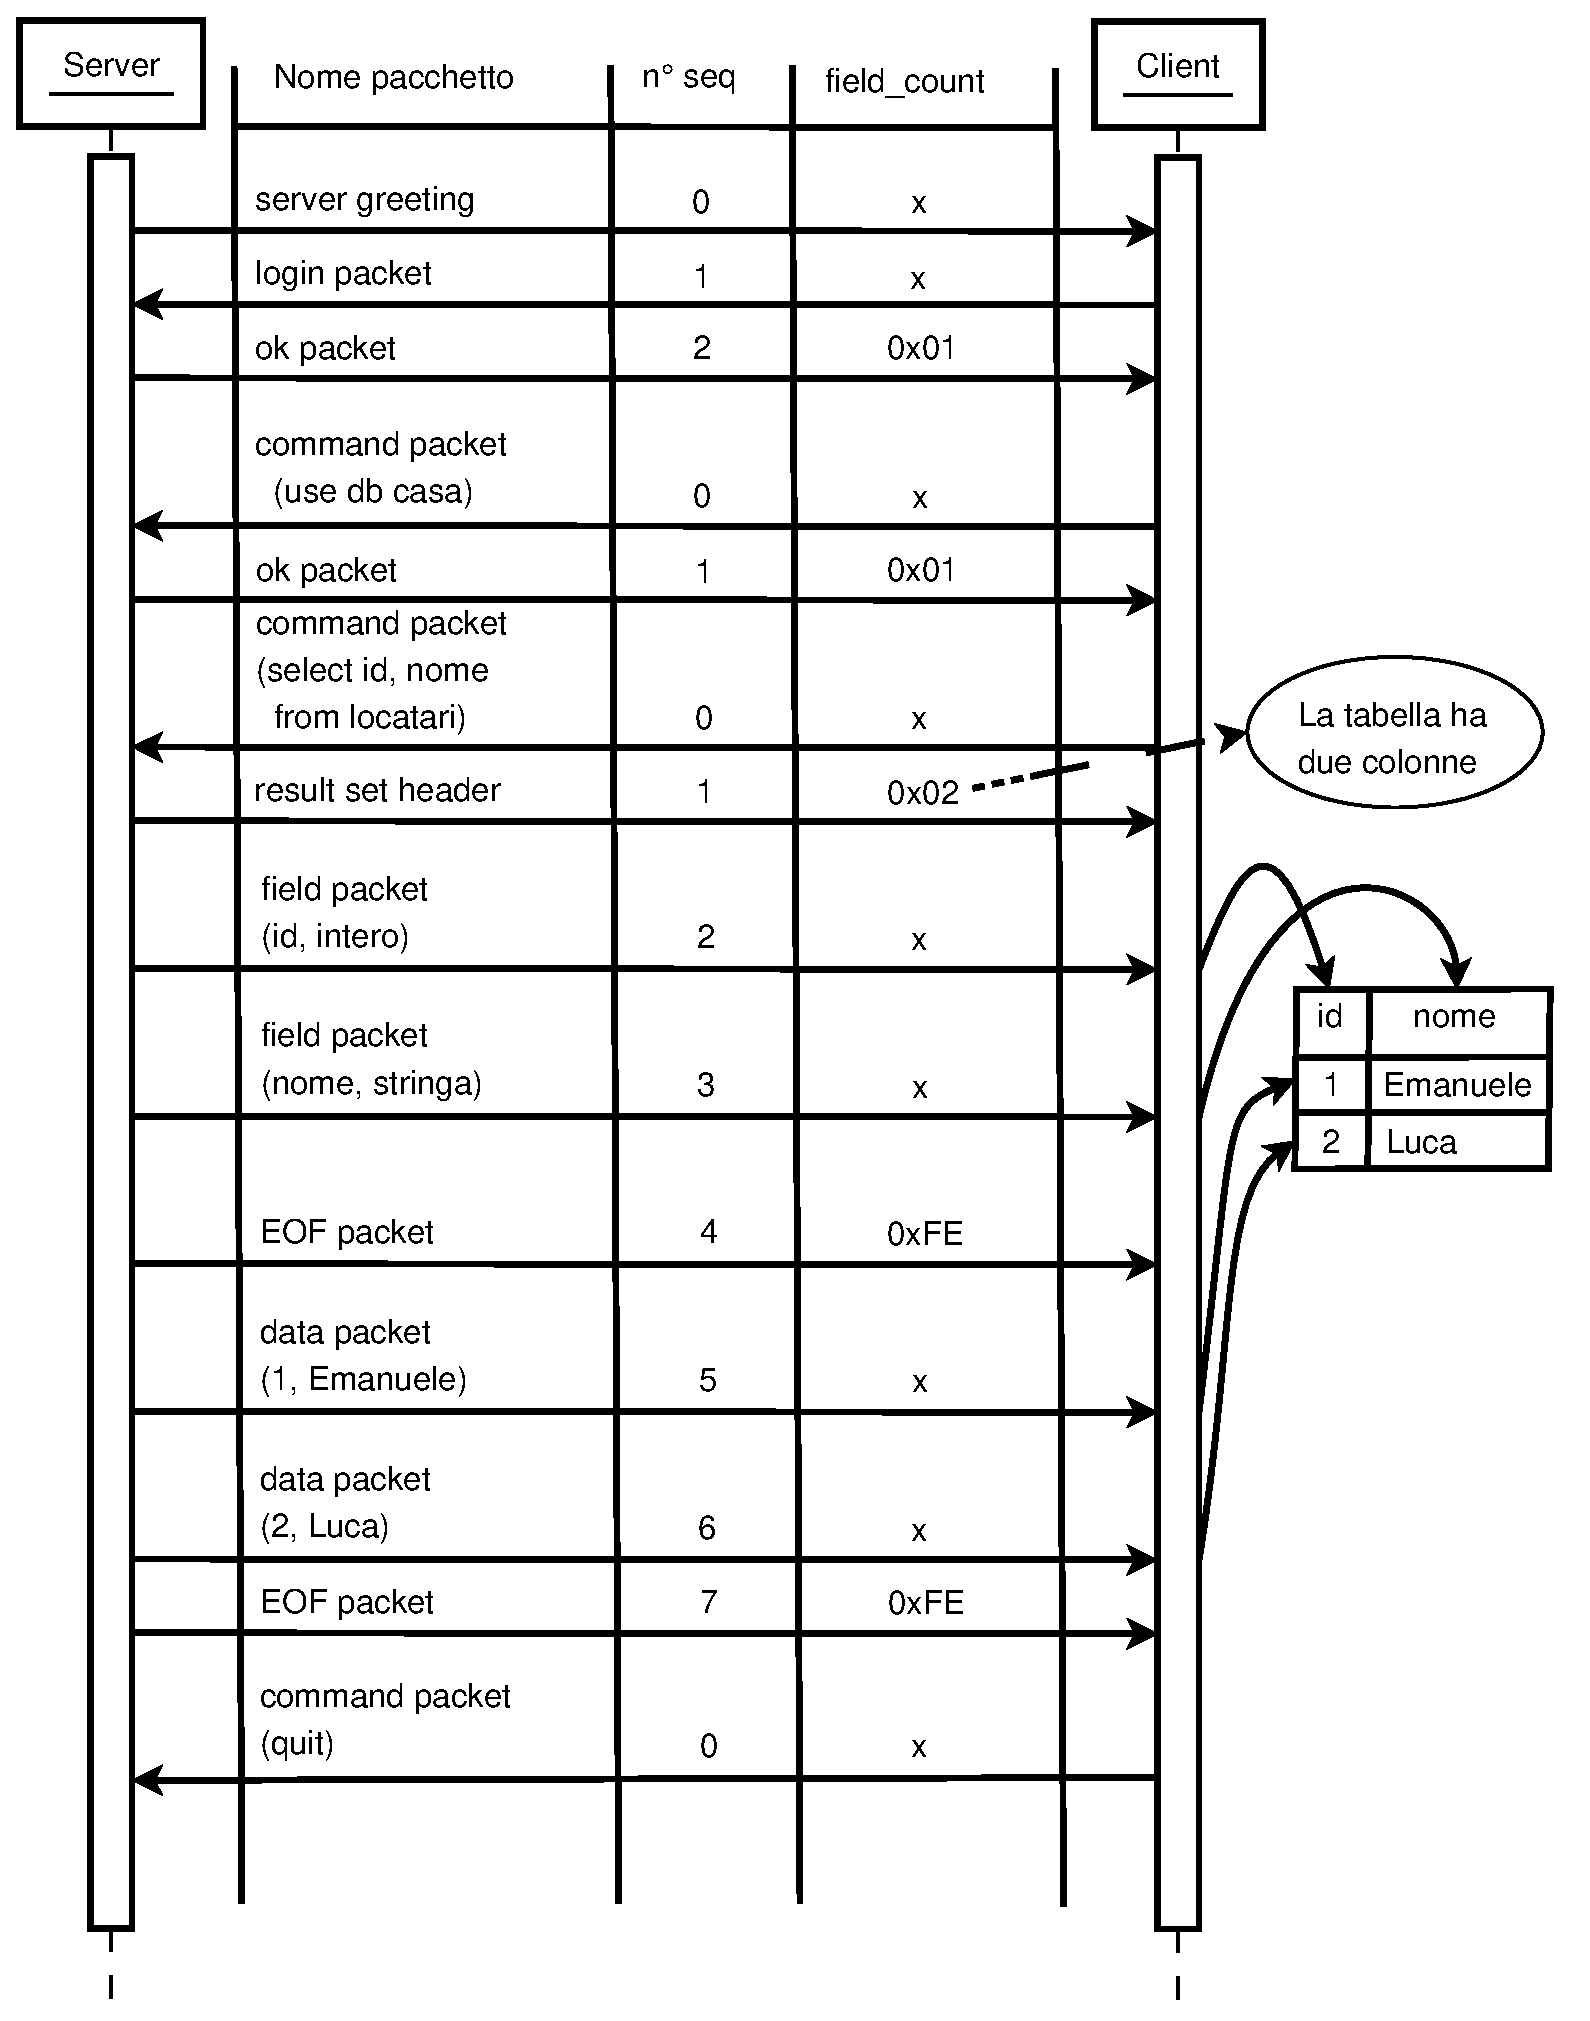
\includegraphics[scale=0.62]{images/mysql_protocol.eps}
    \caption{Esempio di una connessione MySQL}
    \label{mysql-protocol}
\end{figure}

% LocalWords:  MySQL Internals ClientServer Protocol plugin l'username TCP MB
% LocalWords:  L'handshake l'handshake handshake client thread greeting packet
% LocalWords:  username authentication result capabilities L'header riazzerata
% LocalWords:  dell'handshake command field count Error xFF Header query xFD
% LocalWords:  EOF xFE SELECT
